\documentclass[bachelor, och, referat, times]{SCWorks}

% параметр - тип обучения - одно из значений:
%    spec     - специальность
%    bachelor - бакалавриат (по умолчанию)
%    master   - магистратура
% параметр - форма обучения - одно из значений:
%    och   - очное (по умолчанию)
%    zaoch - заочное
% параметр - тип работы - одно из значений:
%    referat    - реферат
%    coursework - курсовая работа (по умолчанию)
%    diploma    - дипломная работа
%    pract      - отчет по практике
%    pract      - отчет о научно-исследовательской работе
%    autoref    - автореферат выпускной работы
%    assignment - задание на выпускную квалификационную работу
%    review     - отзыв руководителя
%    critique   - рецензия на выпускную работу
% параметр - включение шрифта
%    times    - включение шрифта Times New Roman (если установлен)
%               по умолчанию выключен 


\input{preamble.sty}


%убирание преносов слов
\tolerance = 1
\emergencystretch = \maxdimen
\hbadness = 10000

\newcommand{\eqdef}{\stackrel {\rm def}{=}}

\newtheorem{lem}{Лемма}


\begin{document}
    
   % Кафедра (в родительном падеже)
    %\chair{математической кибернетики и компьютерных наук}
    \chair{информатики и программирования}
    % Тема работы
    \title{Использование индексов}
    
    % Курс
    \course{3}
    
    % Группа
    \group{311}
    
    % Факультет (в родительном падеже) (по умолчанию "факультета КНиИТ")
    \department{факультета компьютерных наук и информационных технологий}
    
    % Специальность/направление код - наименование
    
    \napravlenie{02.03.02 "--- Фундаментальная информатика и информационные технологии}
    
    % Для студентки. Для работы студента следующая команда не нужна.
    \studenttitle{студентки}
    
    % Фамилия, имя, отчество в родительном падеже
    \author{Никитенко Яны Валерьевны}
    
    % Заведующий кафедрой 
    %\chtitle{доцент, к.\,ф.-м.\,н.}
    %\chname{С.\,В.\,Миронов}
    % Научный руководитель (для реферата преподаватель проверяющий работу)
    %\satitle{доцент, к.\,ф.-м.\,н.} %должность, степень, звание
    %\saname{А.\,П.\,Грецова}
    % Руководитель ДПП ПП для цифровой кафедры (перекрывает заведующего кафедры)
    % \chpretitle{
    %     заведующий кафедрой математических основ информатики и олимпиадного\\
    %     программирования на базе МАОУ <<Ф"=Т лицей №1>>
    % }
    % \chtitle{г. Саратов, к.\,ф.-м.\,н., доцент}
    % \chname{Кондратова\, Ю.\,Н.}
    \date{2026}
    
    
    % Руководитель практики от организации (руководитель для цифровой кафедры)
    %\patitle{доцент, к.\,ф.-м.\,н.}
    %\paname{С.\,В.\,Миронов}
    
    % Руководитель НИР
    %\nirtitle{доцент, к.\,п.\,н.} % степень, звание
    %\nirname{В.\,А.\,Векслер}
    
    % Семестр (только для практики, для остальных типов работ не используется)
    %\term{2}
    
    % Наименование практики (только для практики, для остальных типов работ не
    % используется)
    %\practtype{учебная}
    
    % Продолжительность практики (количество недель) (только для практики, для
    % остальных типов работ не используется)
    %\duration{2}
    
    % Даты начала и окончания практики (только для практики, для остальных типов
    % работ не используется)
    %\practStart{01.07.2022}
    %\practFinish{13.01.2023}
    
    % Год выполнения отчета
   
    
    \maketitle

    
    
    % Включение нумерации рисунков, формул и таблиц по разделам
    % (по умолчанию - нумерация сквозная)
    % (допускается оба вида нумерации)
    %\secNumbering

    
    
   
    
    % Раздел "Обозначения и сокращения". Может отсутствовать в работе
    %\abbreviations
    %\begin{description}
    %    \item $|A|$  "--- количество элементов в конечном множестве $A$;
    %    \item $\det B$  "--- определитель матрицы $B$;
    %    \item ИНС "--- Искусственная нейронная сеть;
    %    \item FANN "--- Feedforward Artifitial Neural Network
    %\end{description}
    
    % Раздел "Определения". Может отсутствовать в работе
    %\definitions
    
    % Раздел "Определения, обозначения и сокращения". Может отсутствовать в работе.
    % Если присутствует, то заменяет собой разделы "Обозначения и сокращения" и "Определения"
    %\defabbr
    
    \section{Код заполнения таблицы}

{\footnotesize
\begin{verbatim}
    -- Заполнение -- 
-- Клиенты
INSERT INTO Client (Name, LastName, Otchestvo, PhoneNumber, NumberPurchase) VALUES
('Иван', 'Иванов', 'Иванович', '+7(999)123-45-67', 10),
('Мария', 'Петрова', 'Сергеевна', '+7(912)345-67-89', 25),
('Алексей', 'Сидоров', 'Алексеевич', '+7(905)678-90-12', 5),
('Ольга', 'Смирнова', 'Ивановна', '+7(916)234-56-78', 15),
('Дмитрий', 'Кузнецов', 'Дмитриевич', '+7(903)456-78-90', 30),
('Елена', 'Попова', 'Владимировна', '+7(925)567-89-01', 8),
('Сергей', 'Васильев', NULL, '+7(926)678-90-12', 12),
('Анна', 'Павлова', 'Андреевна', '+7(927)789-01-23', 20),
('Андрей', 'Семенов', 'Петрович', '+7(928)890-12-34', 3),
('Наталья', 'Голубева', NULL, '+7(929)901-23-45', 18);
--

-- Старый запрос(он был тестовым, и я решила его оставить)
INSERT INTO Client (Name, LastName, Otchestvo, PhoneNumber, NumberPurchase)
SELECT 
    first_names.name,
    last_names.lastname,
    CASE WHEN random() > 0.3 THEN middle_names.middlename ELSE NULL END,
    '+7(9' || lpad((floor(random() * 100))::text, 2, '0') || ')' || 
    lpad((floor(random() * 1000))::text, 3, '0') || '-' ||
    lpad((floor(random() * 100))::text, 2, '0') || '-' ||
    lpad((floor(random() * 100))::text, 2, '0'),
    floor(random() * 50)
FROM 
    (VALUES ('Петр'), ('Михаил'), ('Владимир'), ('Екатерина'), ('Светлана'),
            ('Татьяна'), ('Юлия'), ('Александр'), ('Николай'), ('Виктор')) first_names(name)
CROSS JOIN 
    (VALUES ('Воробьев'), ('Лебедев'), ('Зайцев'), ('Соловьев'), ('Волков'),
            ('Козлов'), ('Новиков'), ('Морозов'), ('Егоров'), ('Алексеев')) last_names(lastname)
CROSS JOIN 
    (VALUES ('Олегович'), ('Михайлович'), ('Владимирович'), ('Николаевич'),
            ('Олеговна'), ('Михайловна'), ('Владимировна'), ('Николаевна')) middle_names(middlename)
LIMIT 40;

-- Цветы
INSERT INTO Flowers (Species, Name, LatName, Country) VALUES
('Роза', 'Красная роза', 'Rosa rubra', 'Нидерланды'),
('Роза', 'Белая роза', 'Rosa alba', 'Нидерланды'),
('Роза', 'Розовая роза', 'Rosa pink', 'Эквадор'),
('Роза', 'Желтая роза', 'Rosa yellow', 'Кения'),
('Тюльпан', 'Тюльпан красный', 'Tulipa gesneriana', 'Россия'),
('Тюльпан', 'Тюльпан желтый', 'Tulipa yellow', 'Россия'),
('Хризантема', 'Хризантема белая', 'Chrysanthemum', 'Италия'),
('Хризантема', 'Хризантема желтая', 'Chrysanthemum', 'Италия'),
('Пион', 'Пион розовый', 'Paeonia lactiflora', 'Франция'),
('Пион', 'Пион белый', 'Paeonia alba', 'Франция'),
('Гвоздика', 'Гвоздика красная', 'Dianthus', 'Россия'),
('Гортензия', 'Гортензия голубая', 'Hydrangea', 'Япония');
--

-- Букеты
INSERT INTO Bouquet (Name, Quantity, Structure, Price) VALUES
('Романтический', 15, 'Красные розы, зелень', 3500),
('Нежный', 11, 'Белые розы, пионы', 4200),
('Солнечный', 9, 'Желтые тюльпаны, хризантемы', 2800),
('Королевский', 25, 'Розы, пионы, хризантемы', 6500),
('Минимализм', 7, 'Белые хризантемы', 1800),
('Весенний', 13, 'Тюльпаны, нарциссы', 3200),
('Свадебный', 21, 'Белые розы, гортензия', 5500),
('Юбилейный', 31, 'Ассорти из 5 видов цветов', 7800),
('Детский', 9, 'Мелкие разноцветные цветы', 2100),
('Премиум', 51, 'Эксклюзивная композиция', 12500);
--

-- Типы товаров
INSERT INTO TypeGoods (NameType) VALUES
('Букеты'), ('Цветы в упаковке'), ('Горшечные растения'), 
('Сухоцветы'), ('Открытки'), ('Мягкие игрушки'),
('Композиции'), ('Сопутствующие товары');
--

-- Прочее
INSERT INTO AnotherGoods (Name) VALUES
('Роза красная в упаковке'), ('Тюльпаны набор 5 шт'), ('Кактус в горшке'),
('Открытка "С любовью"'), ('Медведь 30 см'), ('Лаванда сухая'),
('Хризантема в горшке'), ('Открытка "С днём рождения"'), ('Зайка мягкая'),
('Букет розовый смешанный'), ('Роза белая в упаковке'), ('Фиалка в горшке'),
('Набор открыток'), ('Собачка мягкая'), ('Эустома в горшке'),
('Композиция в корзине'), ('Ваза стеклянная'), ('Лента упаковочная');
--

-- Цветы и букеты. Связь
INSERT INTO FlowersAndBouquet (IdFlower, IdBouquet) VALUES
-- Романтический (букет 1)
(1, 1), (2, 1),
-- Нежный (букет 2)
(2, 2), (9, 2), (10, 2),
-- Солнечный (букет 3)
(4, 3), (5, 3), (6, 3), (8, 3),
-- Королевский (букет 4)
(1, 4), (3, 4), (7, 4), (9, 4),
-- Минимализм (букет 5)
(7, 5),
-- Весенний (букет 6)
(5, 6), (6, 6),
-- Свадебный (букет 7)
(2, 7), (10, 7), (12, 7),
-- Юбилейный (букет 8)
(1, 8), (3, 8), (7, 8), (9, 8), (11, 8),
-- Детский (букет 9)
(3, 9), (5, 9), (8, 9),
-- Премиум (букет 10)
(1, 10), (3, 10), (9, 10), (12, 10);
--

-- Товары
INSERT INTO Goods (IdAnotherGoods, IdType, IdBouquet) VALUES
-- Тип 1 (Букеты)
(10, 1, 1), (1, 1, 2), (2, 1, 3), (3, 1, 4), (4, 1, 5),
-- Тип 2 (Цветы в упаковке)
(1, 2, NULL), (2, 2, NULL), (11, 2, NULL),
-- Тип 3 (Горшечные растения)
(3, 3, NULL), (7, 3, NULL), (12, 3, NULL), (15, 3, NULL),
-- Тип 4 (Сухоцветы)
(6, 4, NULL),
-- Тип 5 (Открытки)
(4, 5, NULL), (8, 5, NULL), (13, 5, NULL),
-- Тип 6 (Мягкие игрушки)
(5, 6, NULL), (9, 6, NULL), (14, 6, NULL),
-- Тип 7 (Композиции)
(16, 7, NULL),
-- Тип 8 (Сопутствующие товары)
(17, 8, NULL), (18, 8, NULL);
--

-- Чеки
INSERT INTO Account (IdClient, Status, DatePurchase, Summ, ProcentDiscount, SummAll)
SELECT 
    c.Id,
    'оплачено',
    CURRENT_DATE - (floor(random() * 180)::int || ' days')::interval,
    1500 + floor(random() * 10000),
    CASE WHEN random() > 0.7 THEN floor(random() * 20) ELSE 0 END,
    1500 + floor(random() * 10000) * (1 - CASE WHEN random() > 0.7 THEN floor(random() * 20) / 100.0 ELSE 0 END)
FROM Client c
CROSS JOIN generate_series(1, 3) -- по 3 чека на каждого клиента
WHERE c.Id <= 20; -- Для первых 20 клиентов
--

-- Добавление еще активных клиентов
INSERT INTO Account (IdClient, Status, DatePurchase, Summ, ProcentDiscount, SummAll)
SELECT 
    c.Id,
    CASE WHEN random() > 0.9 THEN 'возврат' ELSE 'оплачено' END,
    CURRENT_DATE - (floor(random() * 60)::int || ' days')::interval,
    2000 + floor(random() * 15000),
    CASE WHEN random() > 0.6 THEN floor(random() * 15) ELSE 0 END,
    2000 + floor(random() * 15000) * (1 - CASE WHEN random() > 0.6 THEN floor(random() * 15) / 100.0 ELSE 0 END)
FROM Client c
CROSS JOIN generate_series(1, 2) -- еще по 2 чека
WHERE c.NumberPurchase > 15; -- Только для клиентов с большим числом покупок

-- Товары в чеке
INSERT INTO GoodsCheck (IdCheck, IdAnotherGoods, IdFlower, Price)
SELECT 
    a.Id,
    ag.Id,
    CASE WHEN random() > 0.7 THEN f.Id ELSE NULL END,
    ag.Id * 100 + floor(random() * 1000)
FROM Account a
CROSS JOIN AnotherGoods ag
LEFT JOIN Flowers f ON f.Id = ag.Id % 12 + 1
WHERE random() > 0.7 -- Не для всех товаров, чтобы не было слишком много записей
LIMIT 100;
\end{verbatim}
}

    \section{B-Tree индексы}
        \subsection{Простой B-Tree индекс}
B-tree (сбалансированное дерево) — это самый распространенный тип индекса в PostgreSQL. 
Он поддерживает все стандартные операции сравнения (>, <, >=, <=, =, <>) 
и может использоваться с большинством типов данных. B-tree индексы могут быть использованы 
для сортировки, ограничений уникальности и поиска по диапазону значений. 
Чаще всего они применяются для ускорения операций соединения таблиц (JOIN).


SELECT a.Id, a.DatePurchase, a.Summ, c.Name, c.LastName

FROM Account a

INNER JOIN Client c ON a.IdClient = c.Id;

\begin{figure} [H]
    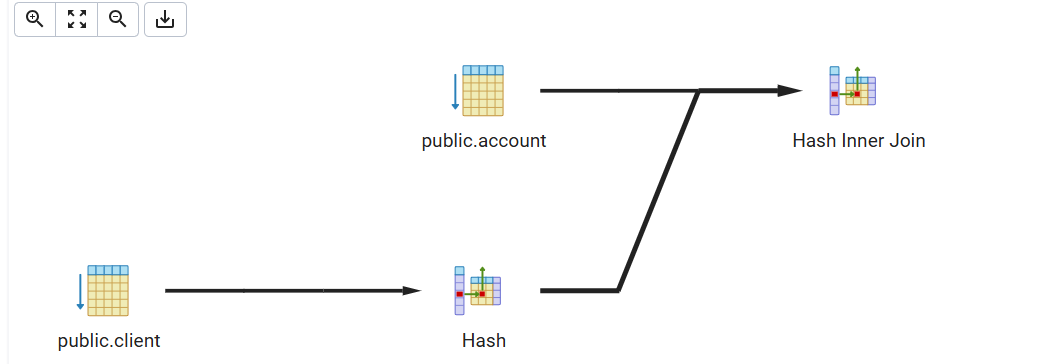
\includegraphics[width=1\textwidth]{Снимок экрана 2026-03-20 110514.png}
\end{figure}


\begin{figure}[H]
    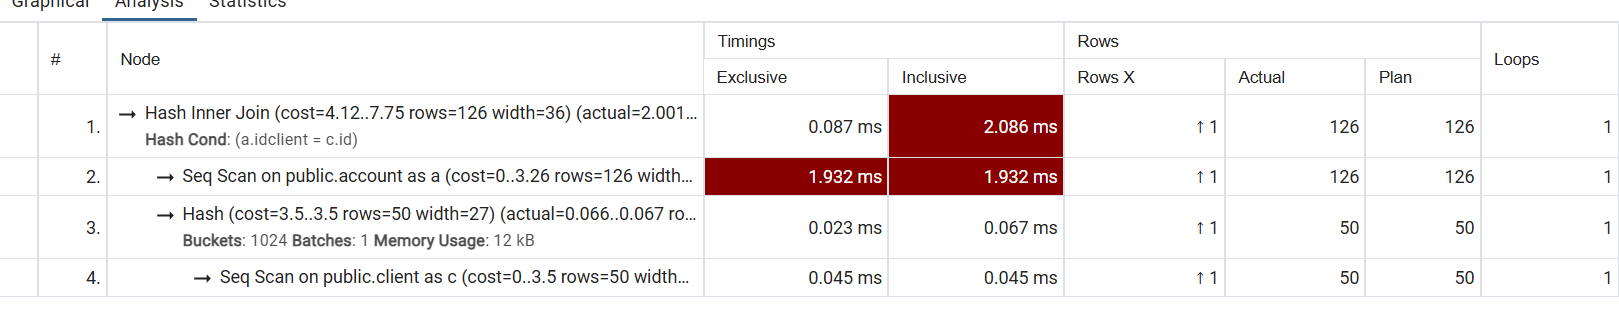
\includegraphics[width=1\textwidth]{Снимок экрана 2026-03-20 110402.png}
\end{figure}



\begin{verbatim}
CREATE INDEX idx_account_idclient_btree ON Account(IdClient);
\end{verbatim}

\begin{figure} [H]
    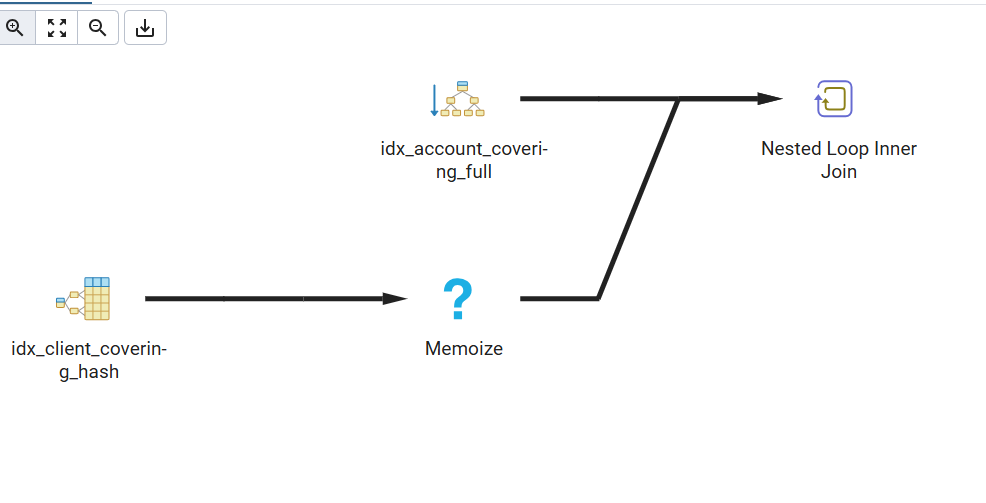
\includegraphics[width=1\textwidth]{Снимок экрана 2026-03-19 221955.png}
\end{figure}


\begin{figure}[H]
    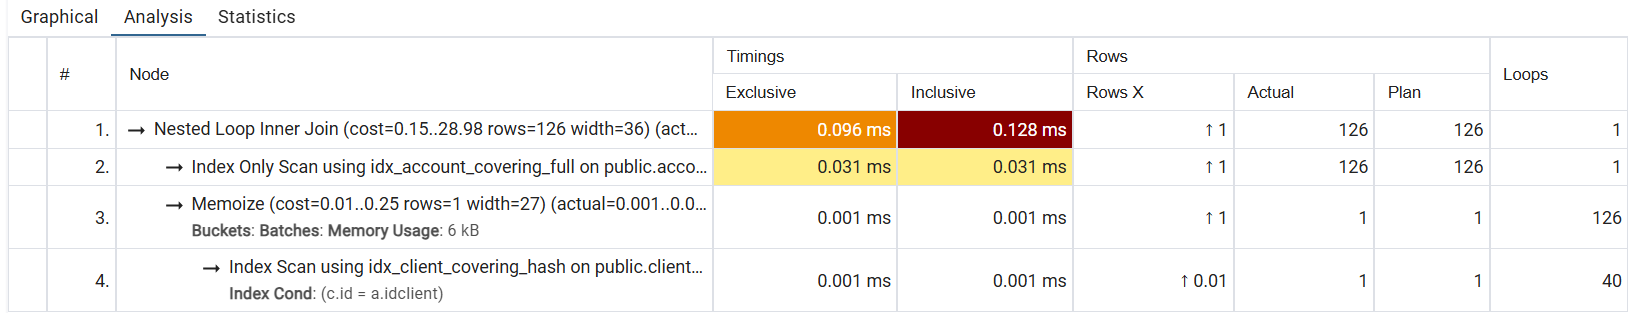
\includegraphics[width=1\textwidth]{Снимок экрана 2026-03-20 002311.png}
\end{figure}



        \subsection{Уникальный B-Tree индекс}

Уникальный B-Tree индекс — это специализированный вариант B-Tree индекса, 
который гарантирует уникальность данных в индексируемых столбцах. 
Помимо ускорения поиска, он обеспечивает целостность данных, 
предотвращая дублирование значений. 
Такой индекс автоматически создаётся при определении ограничения UNIQUE для таблицы.

SELECT Name AS ItemName, 'Flower' AS ItemType FROM Flowers

UNION

SELECT Name, 'Bouquet' FROM Bouquet

ORDER BY ItemName

\begin{figure}[H]
    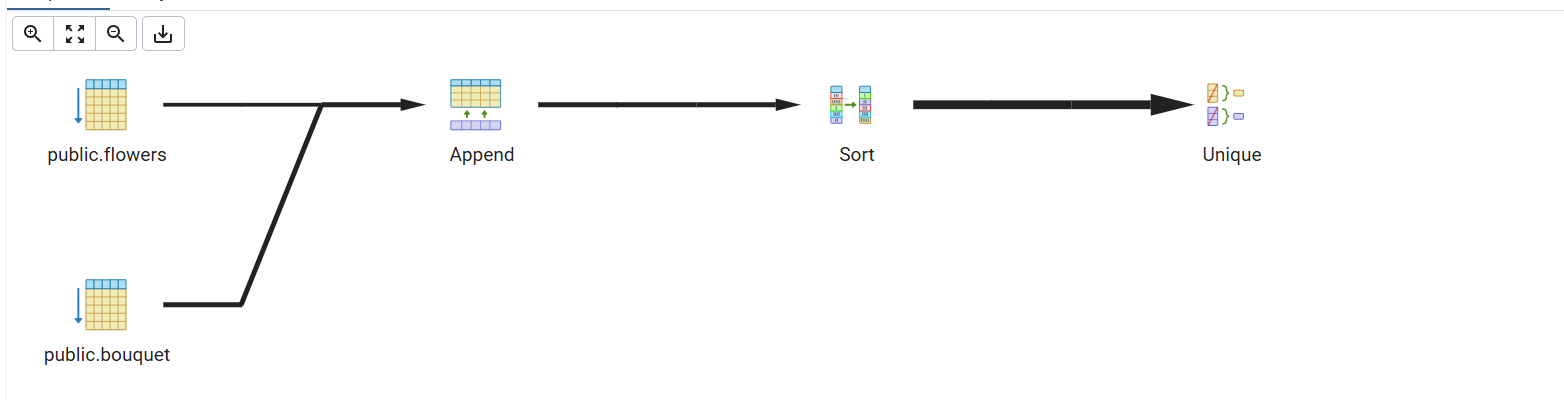
\includegraphics[width=1\textwidth]{Снимок экрана 2026-03-20 110712.png}
\end{figure}

\begin{figure}[H]
    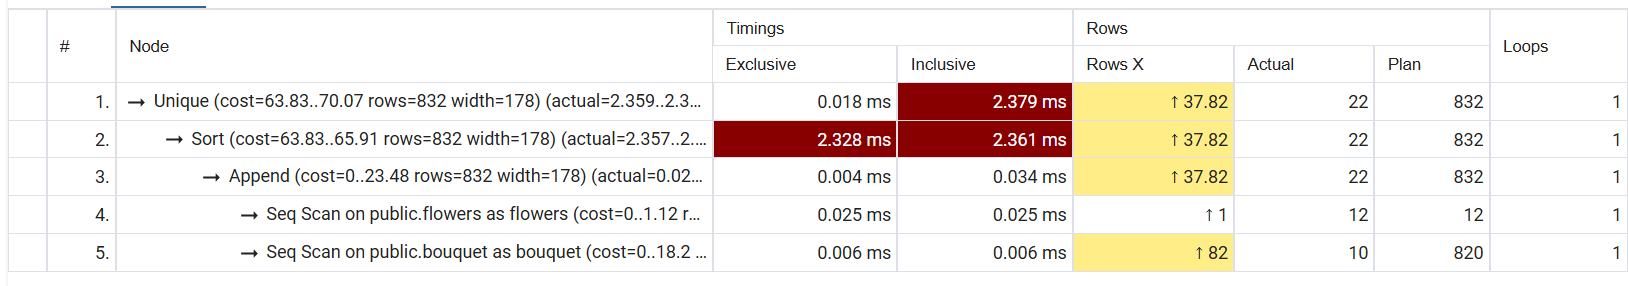
\includegraphics[width=1\textwidth]{Снимок экрана 2026-03-20 110654.png}
\end{figure}



\begin{verbatim}
CREATE UNIQUE INDEX idx_client_phone_unique ON Client(PhoneNumber);
\end{verbatim}

\begin{figure}[H]
    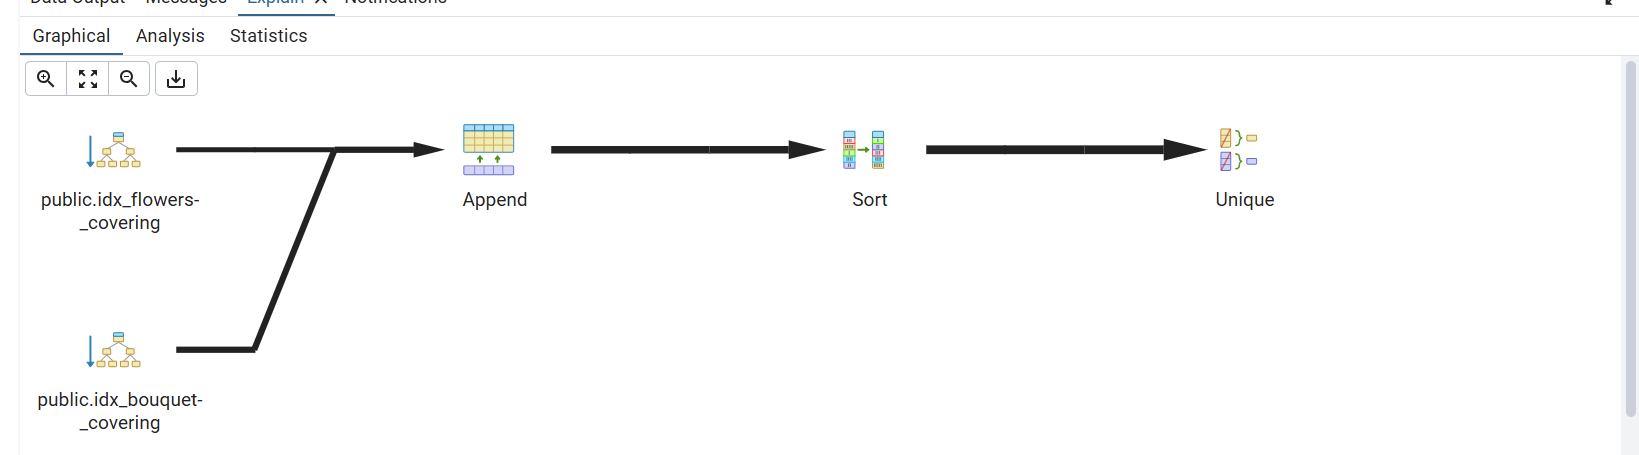
\includegraphics[width=1\textwidth]{Снимок экрана 2026-03-20 002524.png}
\end{figure}

\begin{figure}[H]
    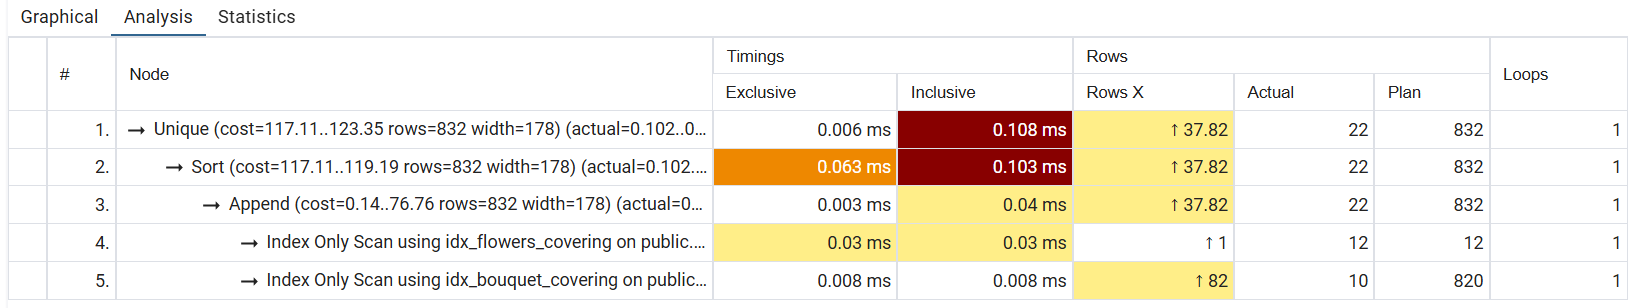
\includegraphics[width=1\textwidth]{Снимок экрана 2026-03-20 002403.png}
\end{figure}


        \subsection{Составной B-Tree индекс}
Составной B-Tree индекс — это индекс, построенный на двух или более 
столбцах таблицы. Он эффективен для запросов, 
которые фильтруют или сортируют по нескольким полям одновременно. 
Порядок столбцов в определении индекса критически важен: 
индекс будет работать для запросов, использующих ведущие (первые) 
столбцы индекса. В данном случае, индекс оптимален для поиска по дате, 
а затем по статусу, или только по дате.

-- Статистика по дням недели

SELECT 

    EXTRACT(DOW FROM DatePurchase) AS DayOfWeek,

    COUNT(*) AS PurchasesCount,

    SUM(Summ) AS TotalSum,

    AVG(Summ)::NUMERIC(10,2) AS AvgSum

FROM Account

WHERE DatePurchase IS NOT NULL

GROUP BY EXTRACT(DOW FROM DatePurchase)

ORDER BY DayOfWeek;

\begin{figure}[H]
    
\includegraphics[width=1\textwidth]{Снимок экрана 2026-03-20 110904.png}
\end{figure}

\begin{figure}[H]
    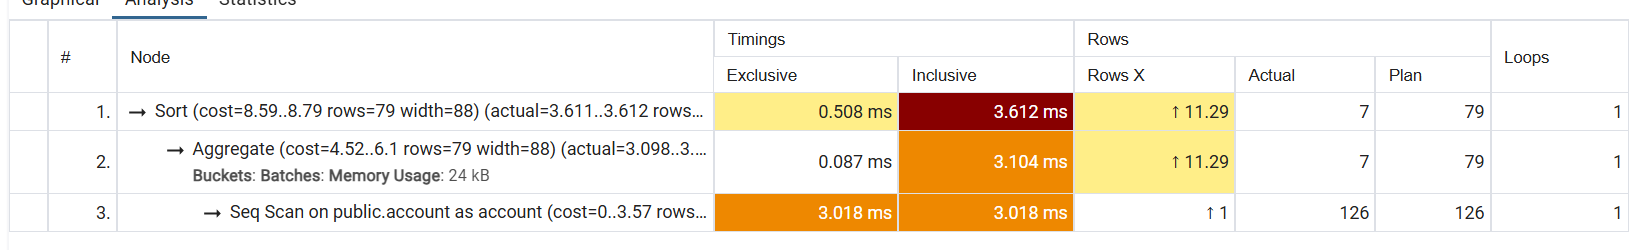
\includegraphics[width=1\textwidth]{Снимок экрана 2026-03-20 110842.png}
\end{figure}


\begin{verbatim}
CREATE INDEX idx_account_date_status_composite ON Account(DatePurchase, Status);
\end{verbatim}


\begin{figure}[H]
    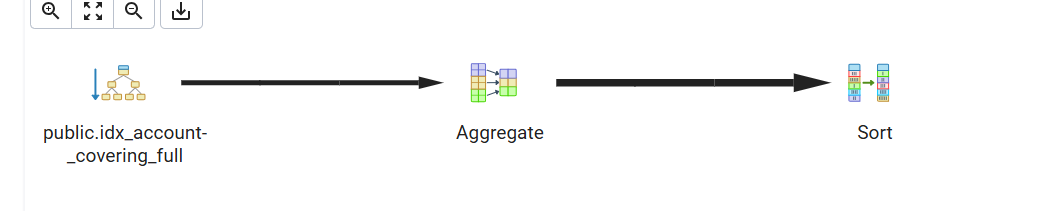
\includegraphics[width=1\textwidth]{Снимок экрана 2026-03-20 005057.png}
\end{figure}

\begin{figure}[H]
    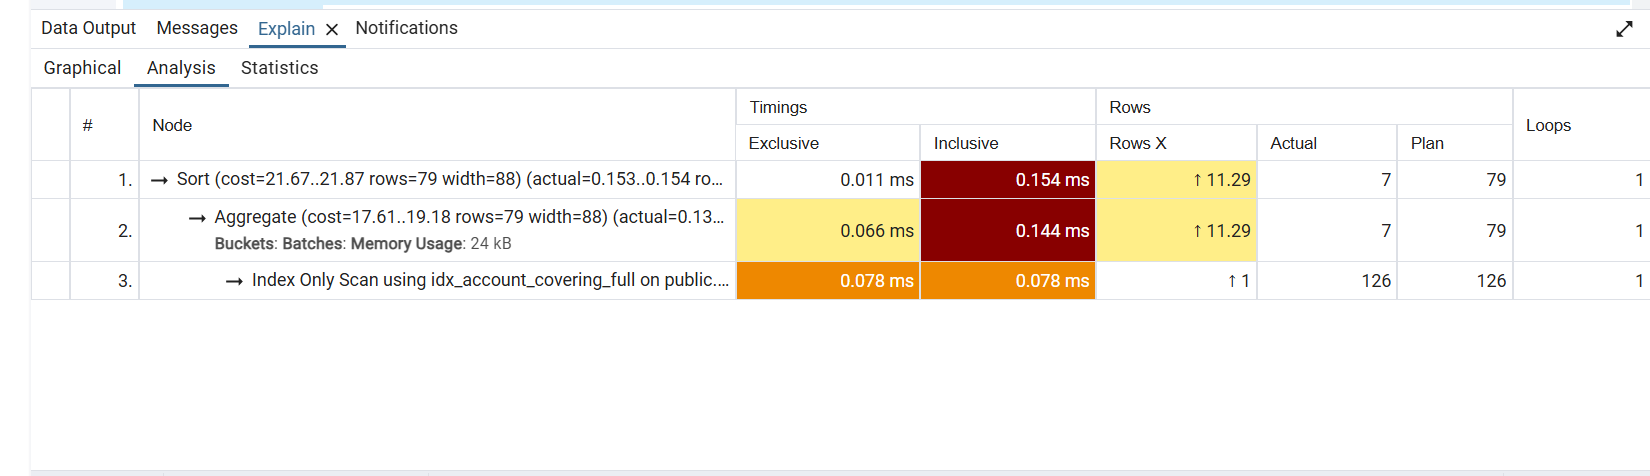
\includegraphics[width=1\textwidth]{Снимок экрана 2026-03-20 004915.png}
\end{figure}


        \subsection{Индекс с выражениями}

SELECT Name AS ItemName, 'Flower' AS ItemType FROM Flowers

UNION

SELECT Name, 'Bouquet' FROM Bouquet

ORDER BY ItemName


\begin{figure}[H]
    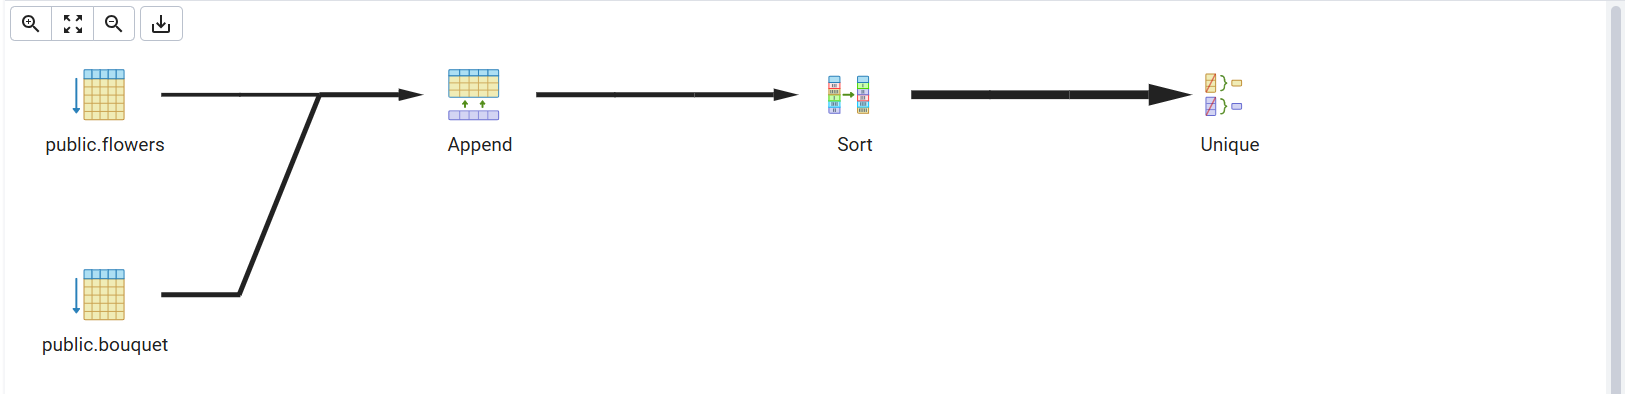
\includegraphics[width=1\textwidth]{Снимок экрана 2026-03-20 111146.png}
\end{figure}

\begin{figure}[H]
    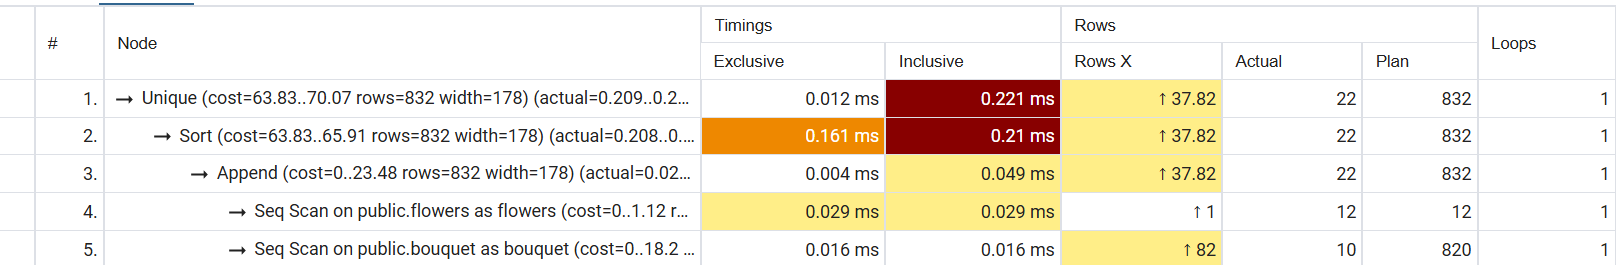
\includegraphics[width=1\textwidth]{Снимок экрана 2026-03-20 111121.png}
\end{figure}
    

\begin{verbatim}
CREATE INDEX idx_flowers_name_upper ON Flowers(UPPER(Name));  
\end{verbatim}


\begin{figure}[H]
    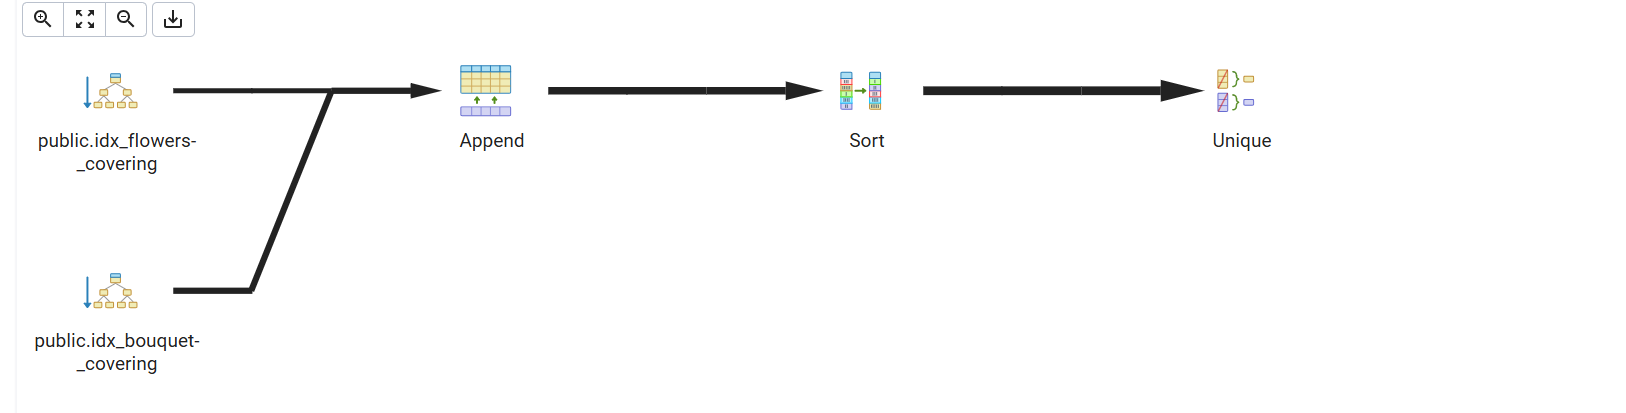
\includegraphics[width=1\textwidth]{Снимок экрана 2026-03-20 005535.png}
\end{figure}

\begin{figure}[H]
    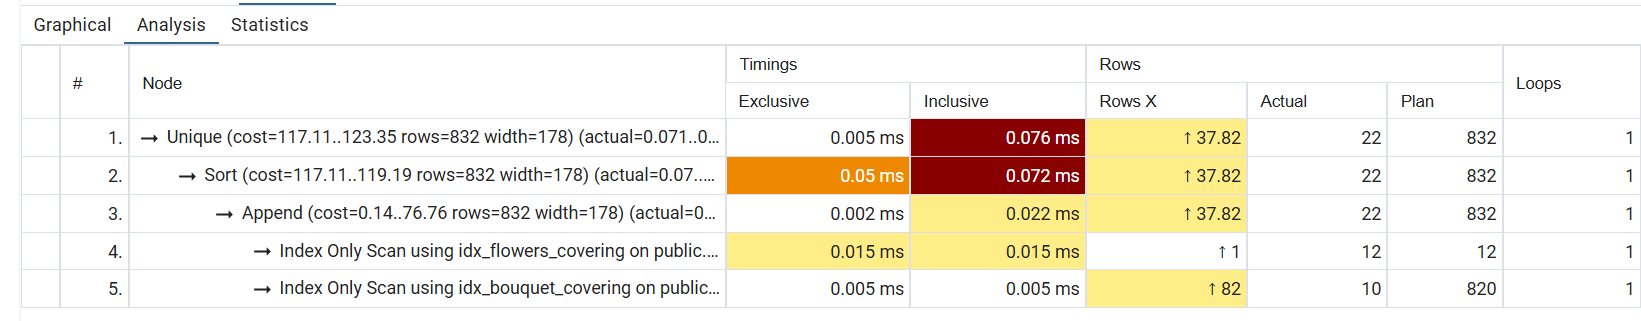
\includegraphics[width=1\textwidth]{Снимок экрана 2026-03-20 005446.png}
\end{figure}

       

        \subsection{Покрывающий индекс}
Покрывающий индекс — это индекс, который содержит все столбцы, 
необходимые для выполнения конкретного запроса. 
Это позволяет выполнить операцию Index Only Scan: 
данные для ответа извлекаются непосредственно из индексной структуры, 
без обращения к основной таблице (heap), что дает максимальную скорость. 
Ключевое слово INCLUDE добавляет в индекс столбцы, которые не участвуют в поиске, 
но нужны для выборки.

\begin{verbatim}
SELECT 
    COALESCE(c.Name, 'Все клиенты') AS ClientName,
    COALESCE(tg.NameType, 'Все типы') AS GoodsType,
    COUNT(*) AS ItemsSold,
    SUM(gc.Price) AS TotalRevenue
FROM GoodsCheck gc
JOIN Account a ON gc.IdCheck = a.Id
JOIN Client c ON a.IdClient = c.Id
JOIN AnotherGoods ag ON gc.IdAnotherGoods = ag.Id
JOIN Goods g ON ag.Id = g.IdAnotherGoods
JOIN TypeGoods tg ON g.IdType = tg.IdTypeGoods
GROUP BY GROUPING SETS (
    (c.Name), -- по клиентам
    (tg.NameType), -- по типам товаров
    (c.Name, tg.NameType), -- по комбинации
    () -- общий итог
)
\end{verbatim}


\begin{figure}[H]
    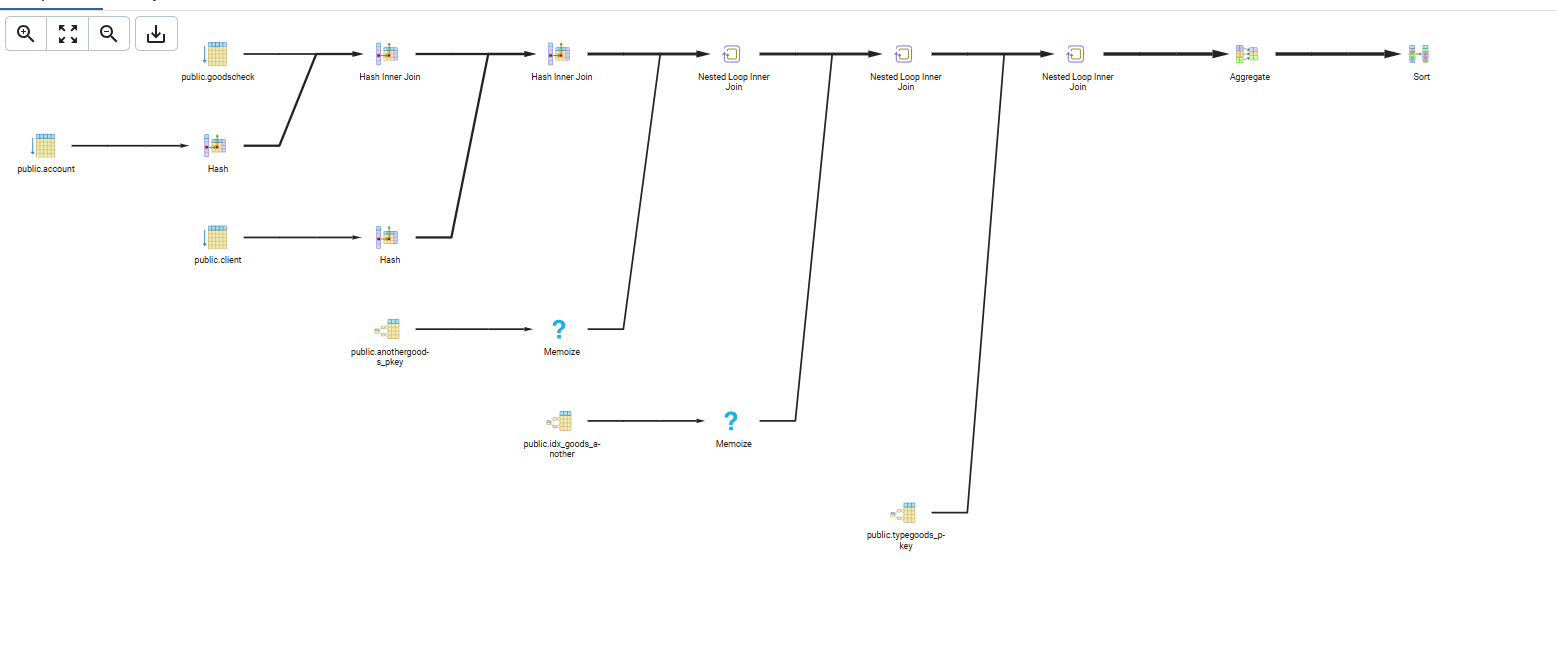
\includegraphics[width=1\textwidth]{Снимок экрана 2026-03-20 111418.png}
\end{figure}


\begin{figure}[H]
    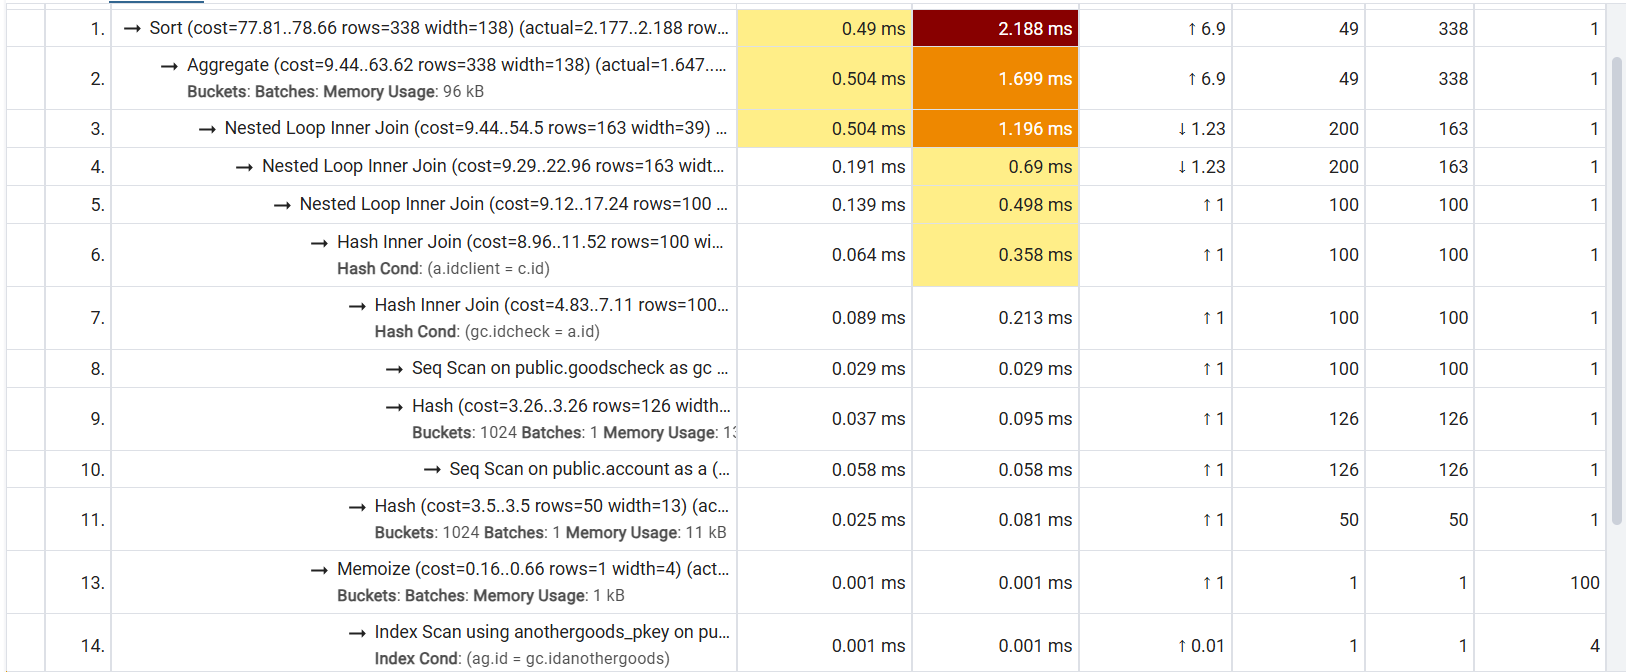
\includegraphics[width=1\textwidth]{Снимок экрана 2026-03-20 111320.png}
\end{figure}
    

\begin{verbatim}
CREATE INDEX idx_typegoods_covering ON TypeGoods(IdTypeGoods, NameType)
INCLUDE ();
\end{verbatim}

\begin{figure}[H]
    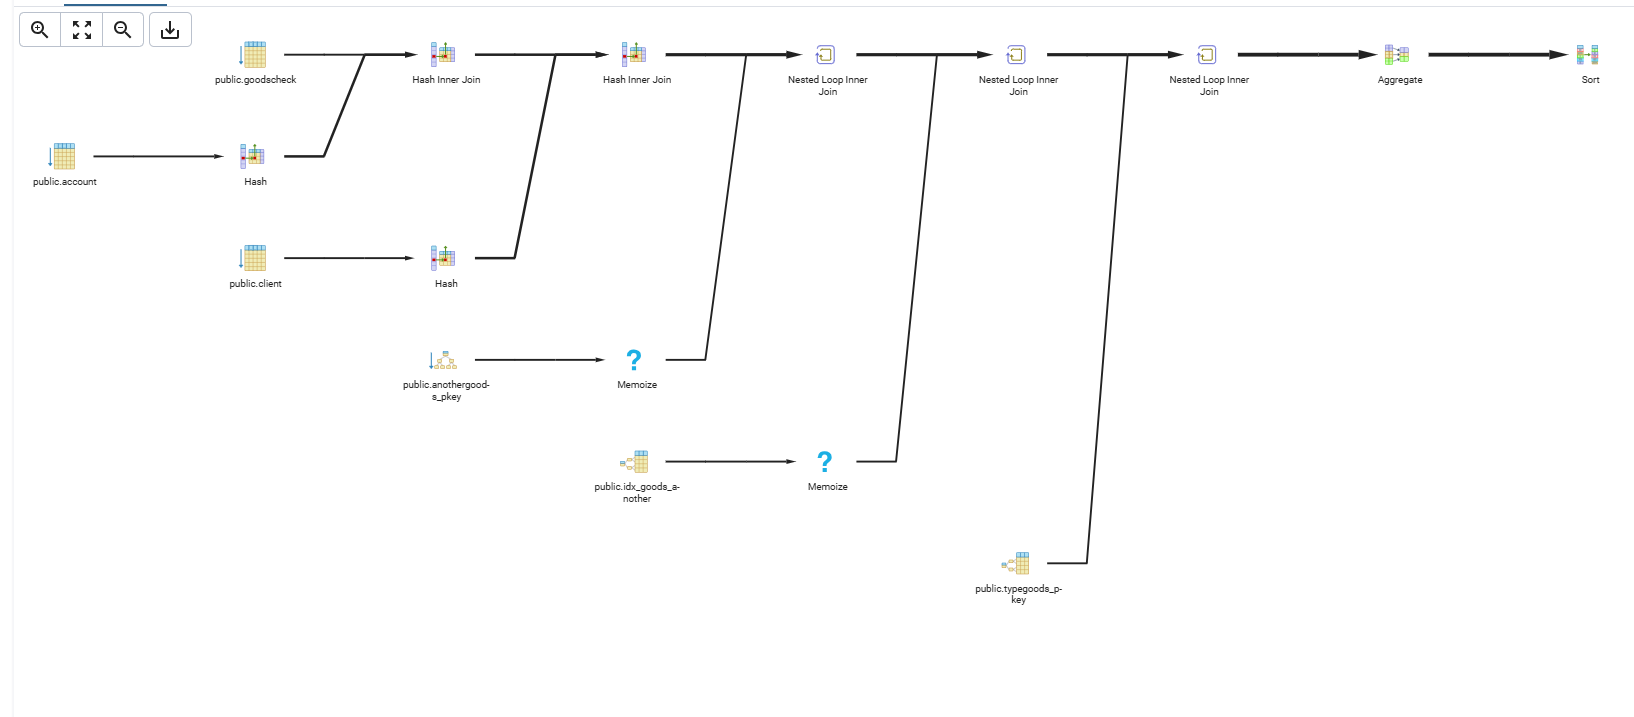
\includegraphics[width=1\textwidth]{Снимок экрана 2026-03-20 101001.png}
\end{figure}


\begin{figure}[H]
    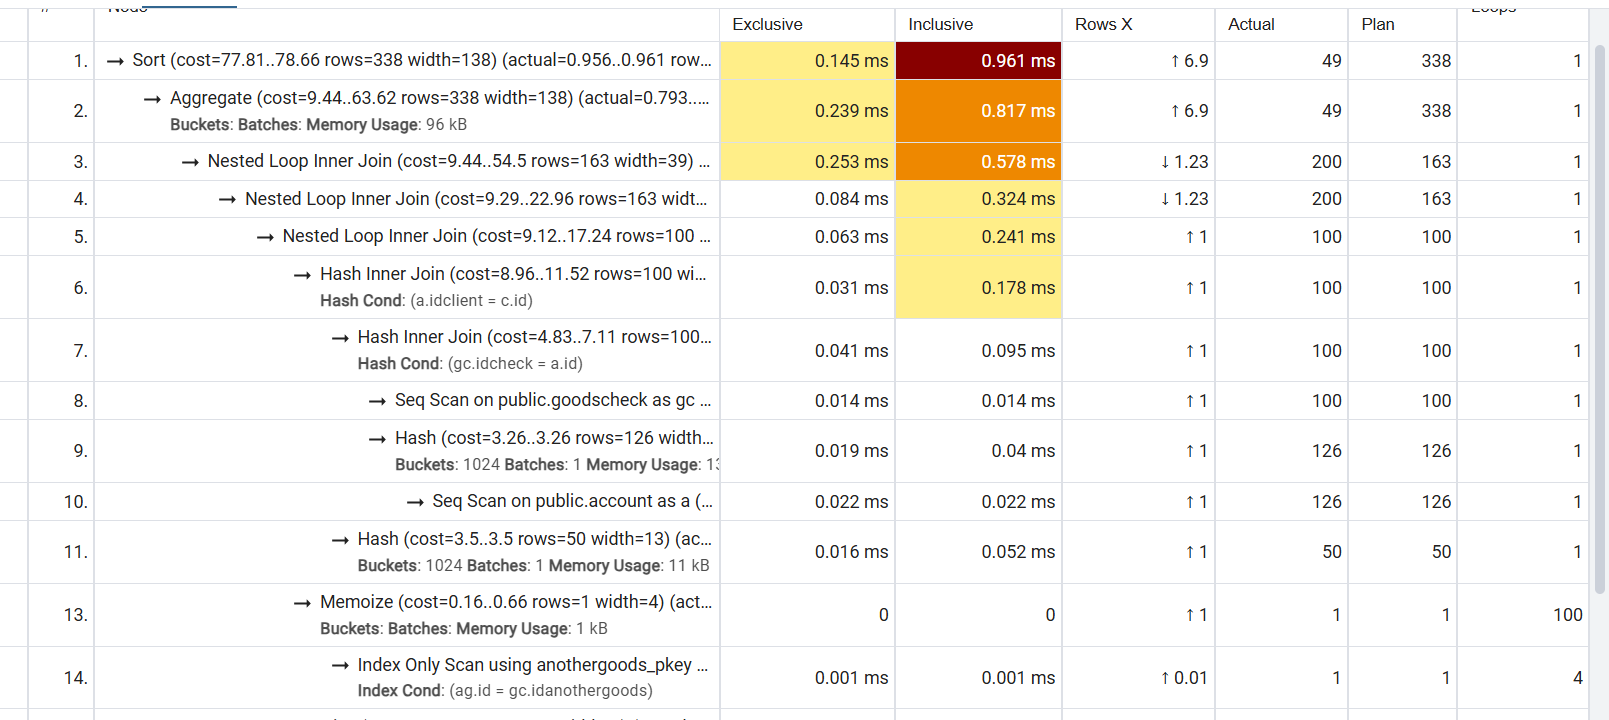
\includegraphics[width=1\textwidth]{Снимок экрана 2026-03-20 100917.png}
\end{figure}
 
        \subsection{Частичный индекс}
Частичный индекс — это индекс, построенный только для подмножества строк таблицы, 
которые удовлетворяют заданному условию (WHERE). 
Он меньше по размеру и часто эффективнее для запросов, 
соответствующих этому условию, так как индексирует только интересующую 
нас часть таблицы.

        
  \begin{verbatim}
  SELECT 
    c.Name || ' ' || c.LastName AS FullName,
    COUNT(*) AS TotalPurchases,
    COUNT(*) FILTER (WHERE a.Summ < 2000) AS SmallPurchases,
    COUNT(*) FILTER (WHERE a.Summ BETWEEN 2000 AND 5000) AS MediumPurchases,
    COUNT(*) FILTER (WHERE a.Summ > 5000) AS LargePurchases,
    SUM(a.Summ) FILTER (WHERE a.Status = 'возврат') AS ReturnedSum,
    SUM(a.Summ) FILTER (WHERE a.Status = 'оплачено') AS PaidSum,
    AVG(a.Summ) FILTER (WHERE a.ProcentDiscount > 0)::NUMERIC(10,2) AS AvgCheckWithDiscount
FROM Client c
JOIN Account a ON c.Id = a.IdClient
GROUP BY c.Id, c.Name, c.LastName
HAVING COUNT(*) > 0
ORDER BY TotalPurchases DESC
LIMIT 15;  
  \end{verbatim}


   \begin{figure}[H]
    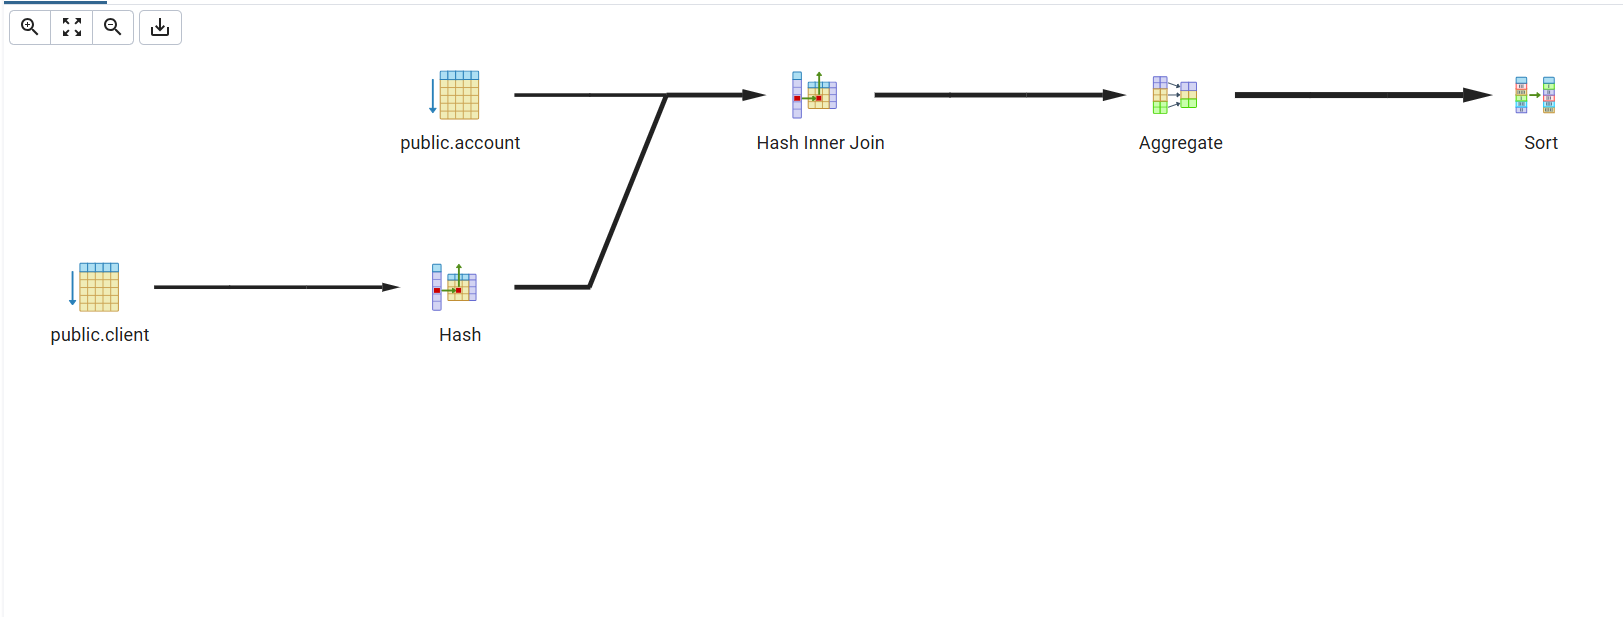
\includegraphics[width=1\textwidth]{Снимок экрана 2026-03-20 111656.png}
\end{figure}


\begin{figure}[H]
    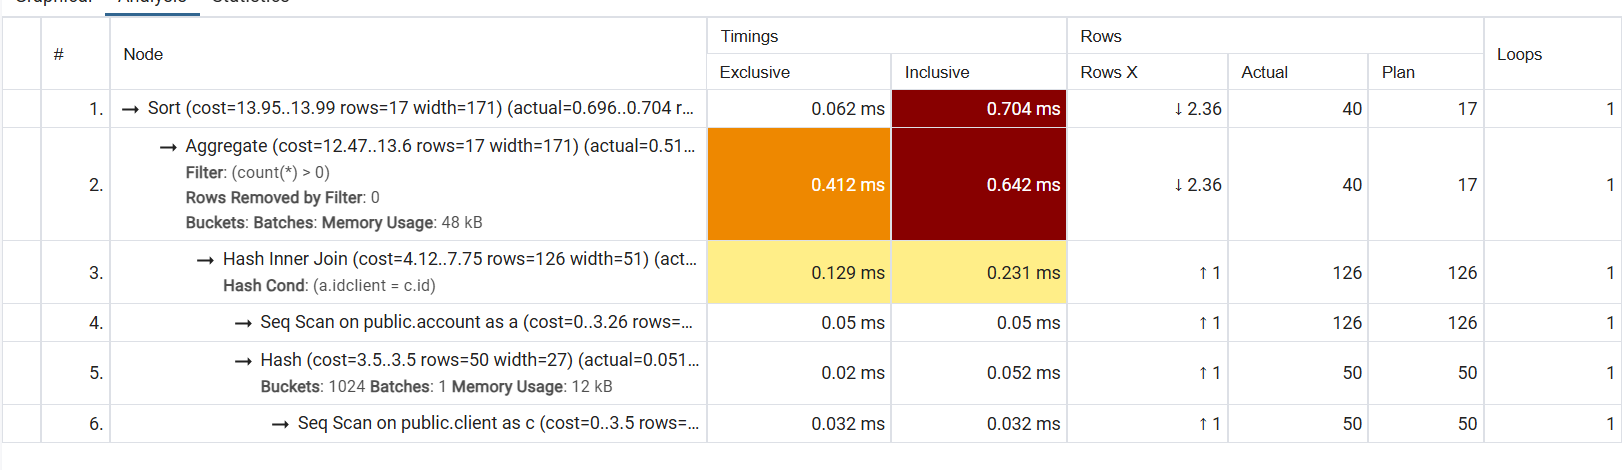
\includegraphics[width=1\textwidth]{Снимок экрана 2026-03-20 111556.png}
\end{figure}


  \begin{verbatim}
 CREATE INDEX idx_client_vip_partial ON Client(Id, Name, LastName, NumberPurchase) 
WHERE NumberPurchase > 25;   
  \end{verbatim}


  \begin{figure}[H]
    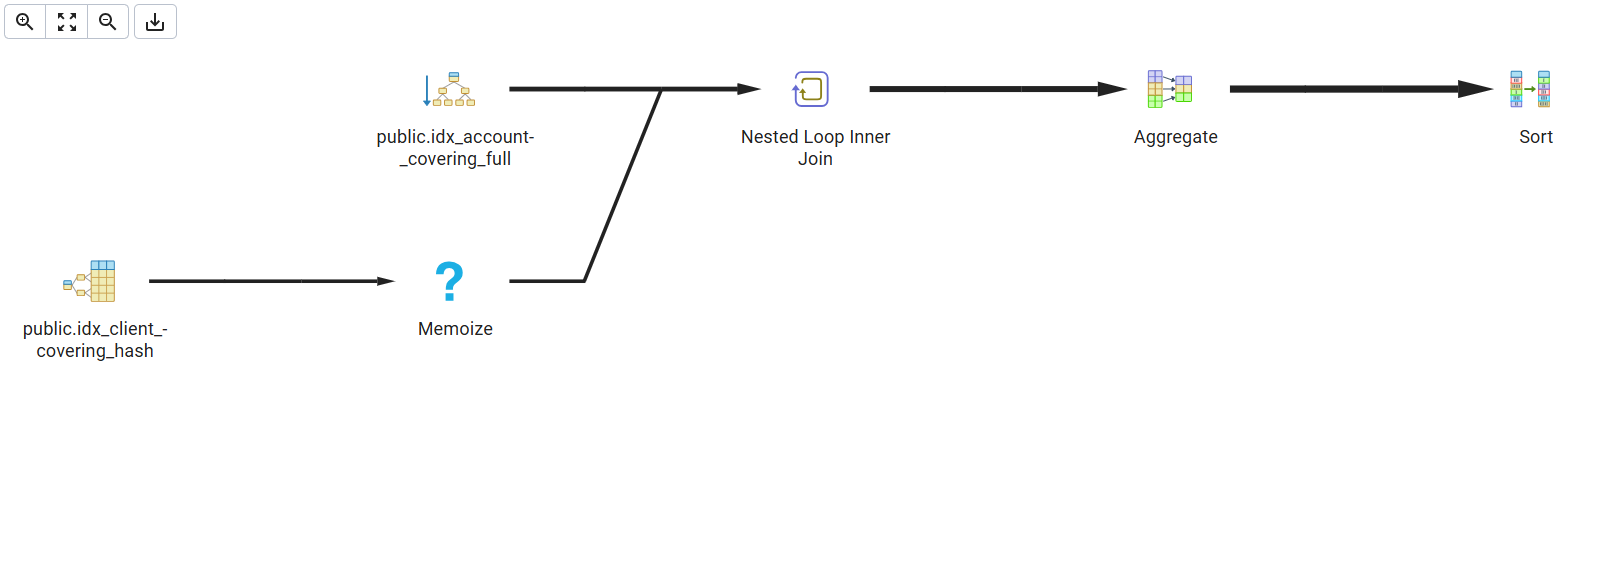
\includegraphics[width=1\textwidth]{Снимок экрана 2026-03-20 102015.png}
\end{figure}


\begin{figure}[H]
    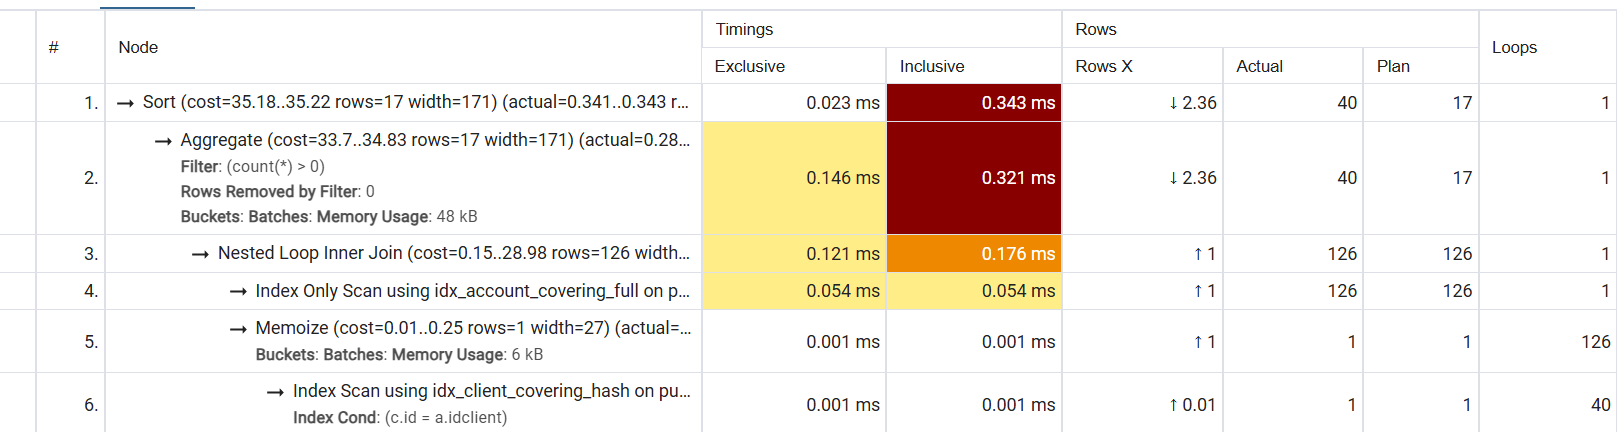
\includegraphics[width=1\textwidth]{Снимок экрана 2026-03-20 101917.png}
\end{figure}


        \subsection{Частичный покрывающий индекс}
Это комбинация частичного индекса и покрывающего индекса 
(с использованием ключевого слова INCLUDE). 
Он создает небольшой и эффективный индекс только для определенного 
подмножества строк (например, для самых ценных клиентов), 
который при этом содержит все данные для запроса, исключая обращение к таблице.

\begin{verbatim}
SELECT 
    CASE 
        WHEN c.NumberPurchase < 10 THEN 'Новичок'
        WHEN c.NumberPurchase < 20 THEN 'Регулярный'
        WHEN c.NumberPurchase < 30 THEN 'Постоянный'
        ELSE 'VIP'
    END AS ClientCategory,
    COUNT(DISTINCT c.Id) AS ClientCount,
    COUNT(a.Id) AS TotalPurchases,
    SUM(a.Summ) AS TotalSpent,
    AVG(a.Summ)::NUMERIC(10,2) AS AvgCheck,
    SUM(a.Summ) / NULLIF(COUNT(DISTINCT c.Id), 0)::NUMERIC(10,2) AS SpentPerClient
FROM Client c
LEFT JOIN Account a ON c.Id = a.IdClient
GROUP BY 
    CASE 
        WHEN c.NumberPurchase < 10 THEN 'Новичок'
        WHEN c.NumberPurchase < 20 THEN 'Регулярный'
        WHEN c.NumberPurchase < 30 THEN 'Постоянный'
        ELSE 'VIP'
    END
ORDER BY 
    MIN(c.NumberPurchase);
\end{verbatim}

 \begin{figure}[H]
    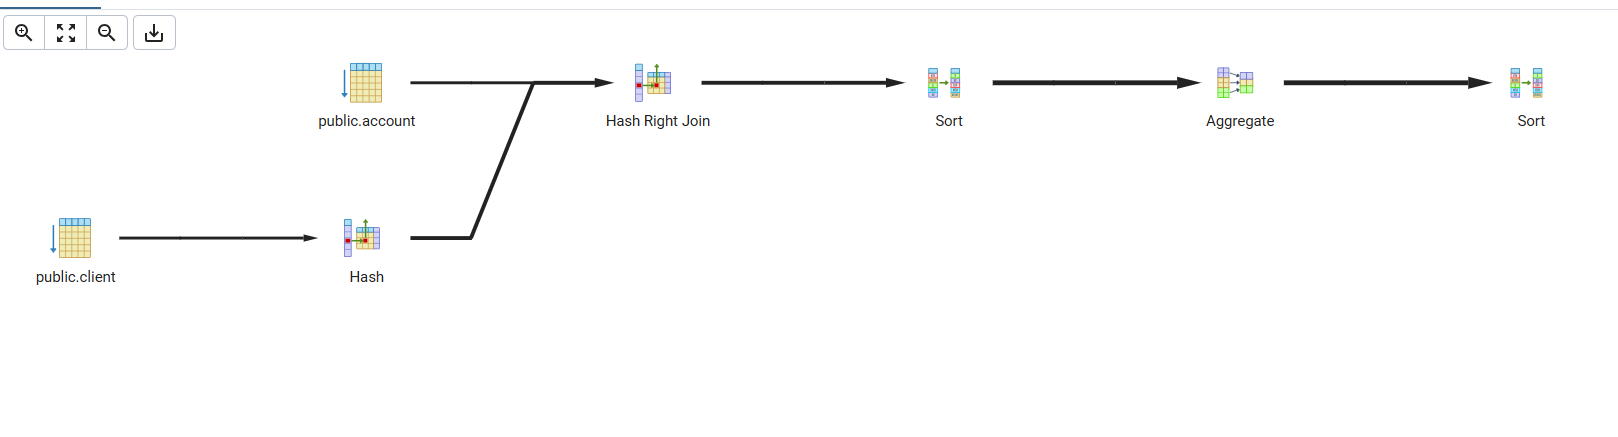
\includegraphics[width=1\textwidth]{Снимок экрана 2026-03-20 112222.png}
\end{figure}


\begin{figure}[H]
    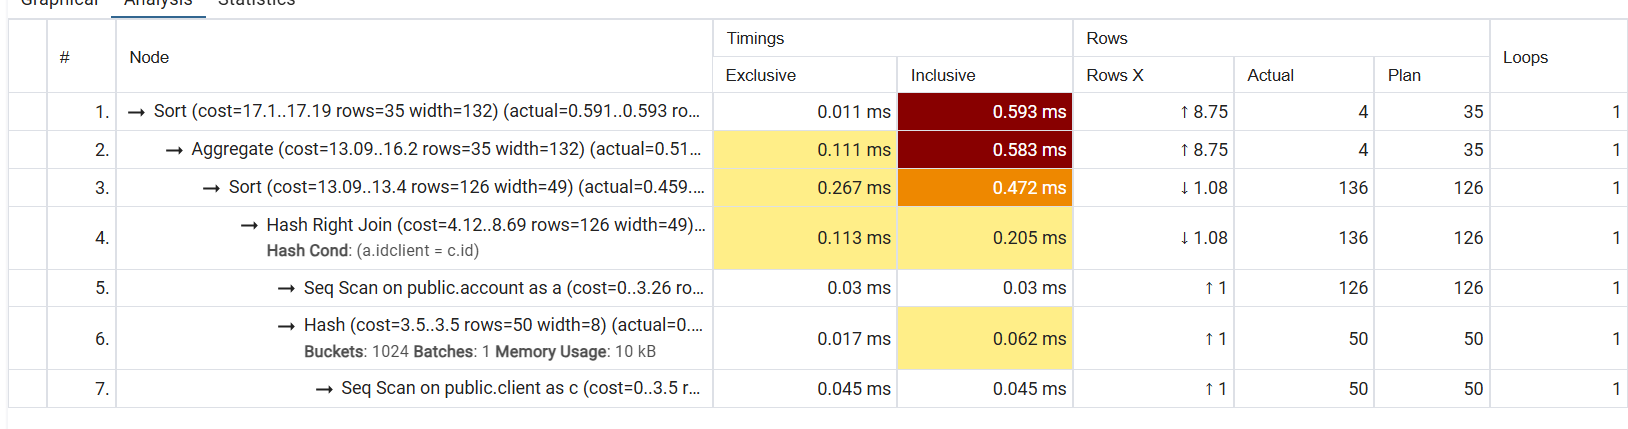
\includegraphics[width=1\textwidth]{Снимок экрана 2026-03-20 112204.png}
\end{figure}



\begin{verbatim}
CREATE INDEX idx_client_vip_covering_partial ON Client(Id, Name, LastName, NumberPurchase) 
INCLUDE (Otchestvo, PhoneNumber) 
WHERE NumberPurchase > 25;
\end{verbatim}


  \begin{figure}[H]
    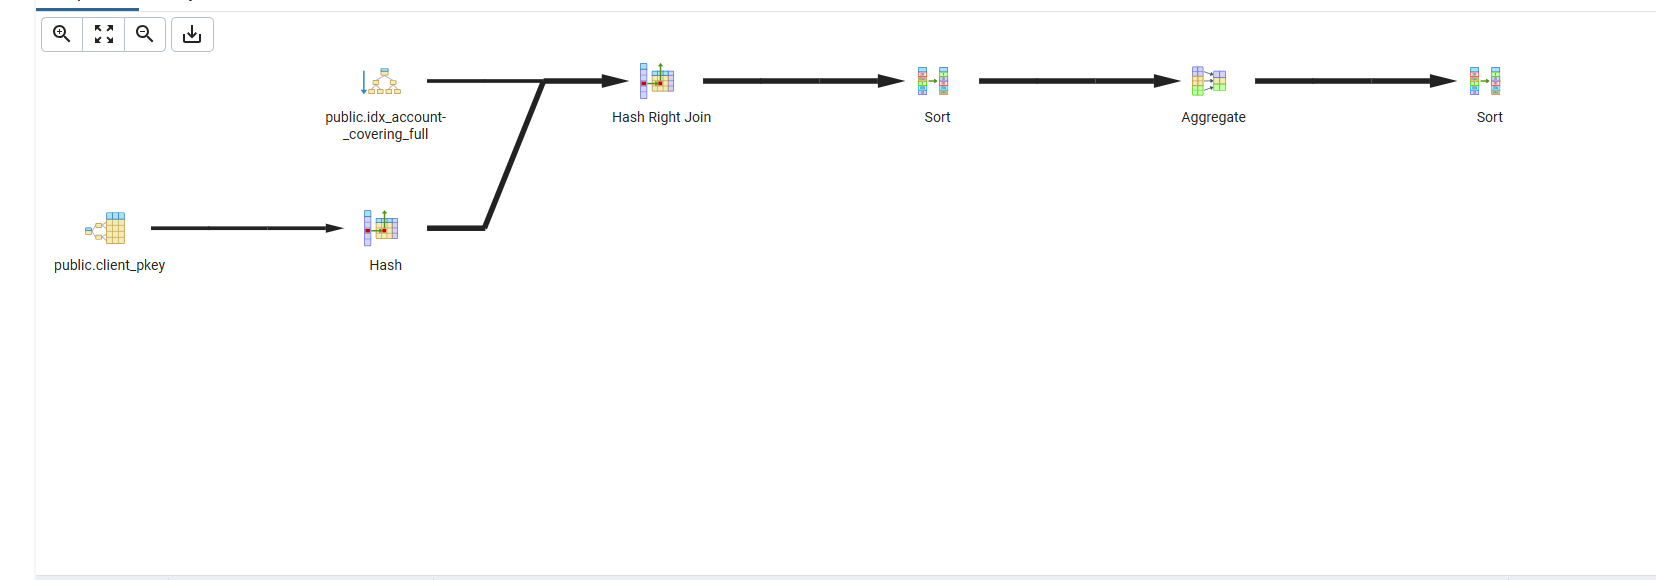
\includegraphics[width=1\textwidth]{Снимок экрана 2026-03-20 105954.png}
\end{figure}


\begin{figure}[H]
    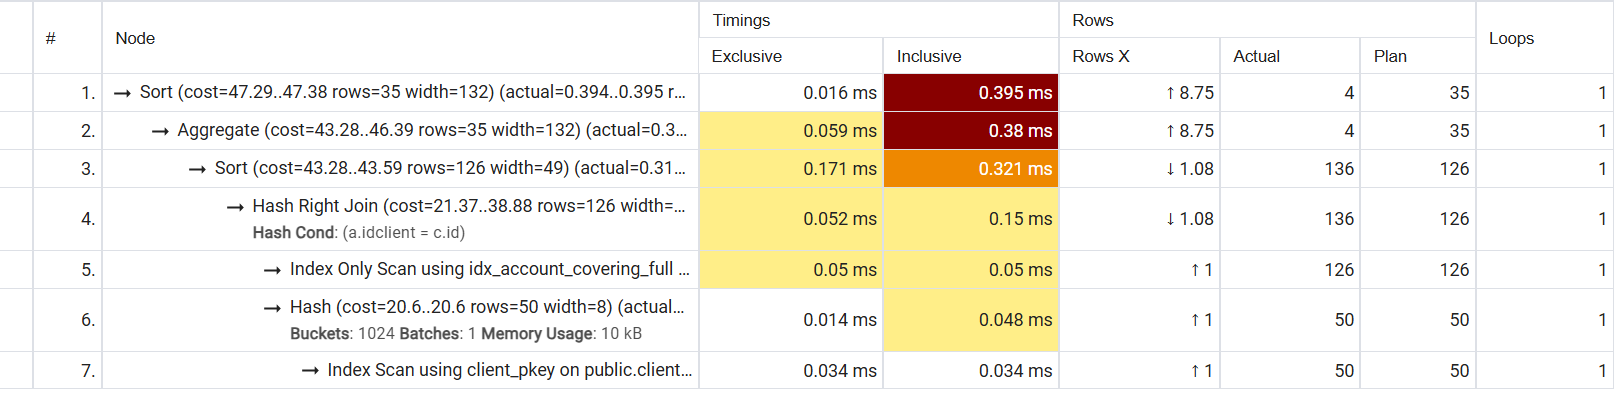
\includegraphics[width=1\textwidth]{Снимок экрана 2026-03-20 105911.png}
\end{figure}

    \section{Hash индексы}
    \subsection{Простой Hash индекс}


      \begin{verbatim}
SELECT 
    c.Name || ' ' || c.LastName AS FullName,
    COUNT(*) AS TotalPurchases,
    COUNT(*) FILTER (WHERE a.Summ < 2000) AS SmallPurchases,
    COUNT(*) FILTER (WHERE a.Summ BETWEEN 2000 AND 5000) AS MediumPurchases,
    COUNT(*) FILTER (WHERE a.Summ > 5000) AS LargePurchases,
    SUM(a.Summ) FILTER (WHERE a.Status = 'возврат') AS ReturnedSum,    
    SUM(a.Summ) FILTER (WHERE a.Status = 'оплачено') AS PaidSum,     
    AVG(a.Summ) FILTER (WHERE a.ProcentDiscount > 0)::NUMERIC(10,2) AS AvgCheckWithDiscount
FROM Client c
JOIN Account a ON c.Id = a.IdClient
GROUP BY c.Id, c.Name, c.LastName
HAVING COUNT(*) > 0
ORDER BY TotalPurchases DESC; 
  \end{verbatim}


   \begin{figure}[H]
    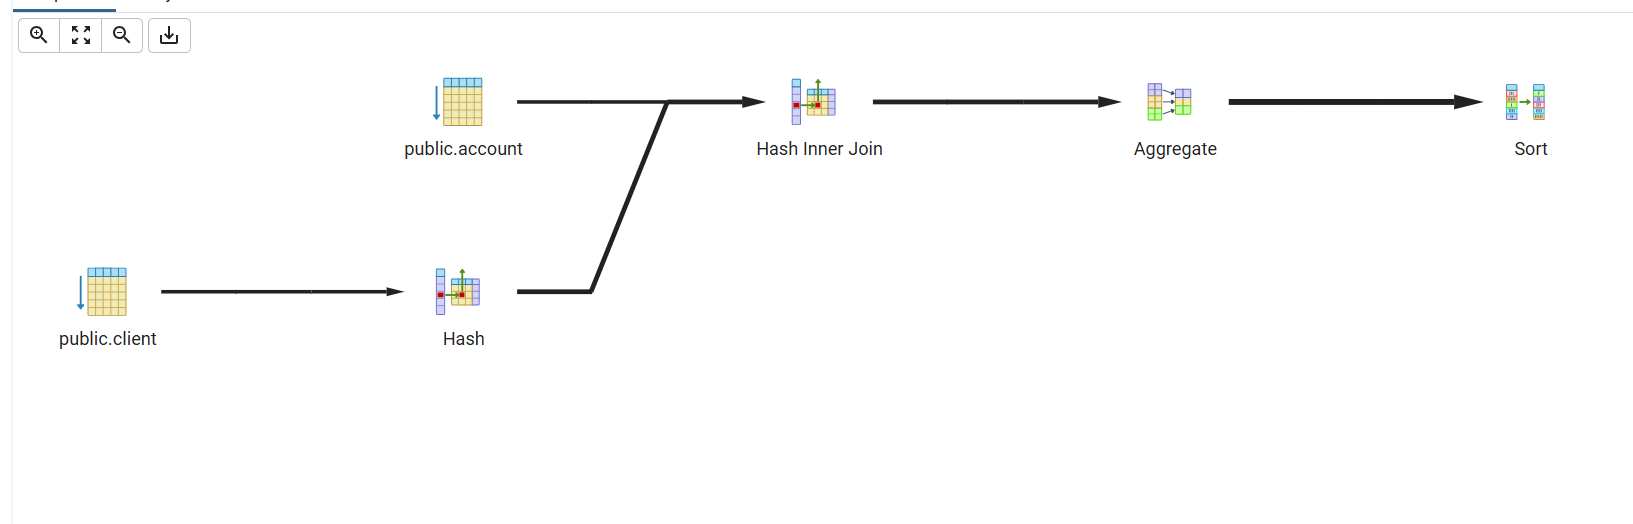
\includegraphics[width=1\textwidth]{Снимок экрана 2026-03-20 112522.png}
\end{figure}


\begin{figure}[H]
    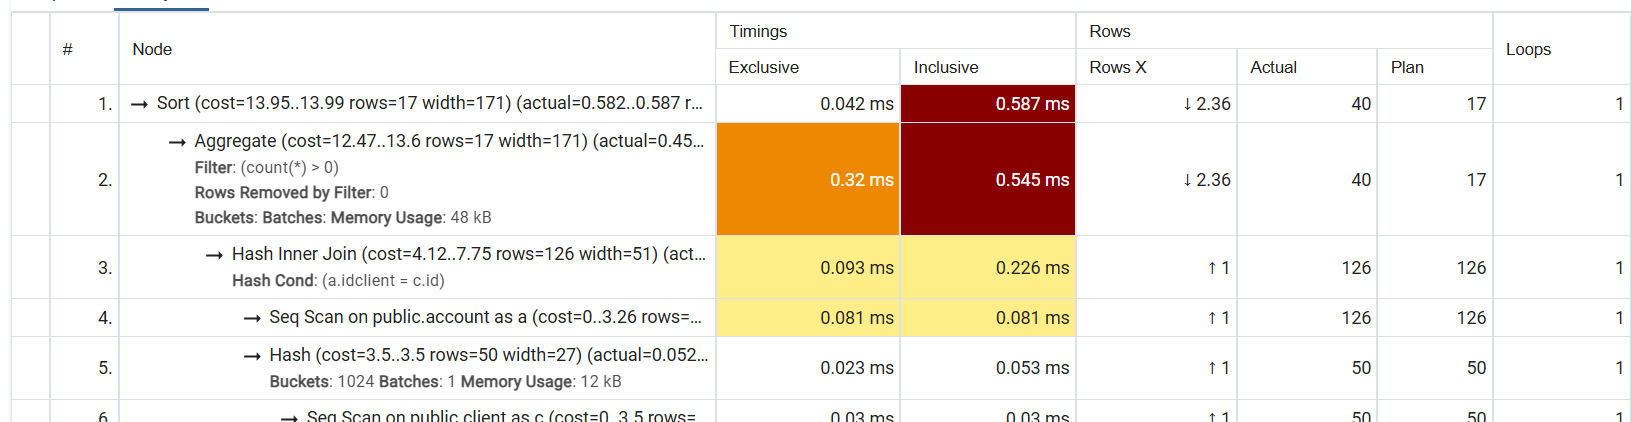
\includegraphics[width=1\textwidth]{Снимок экрана 2026-03-20 112439.png}
\end{figure}


  \begin{verbatim}
CREATE INDEX idx_account_status_hash ON Account USING HASH(Status);
  \end{verbatim}

  \begin{figure}[H]
    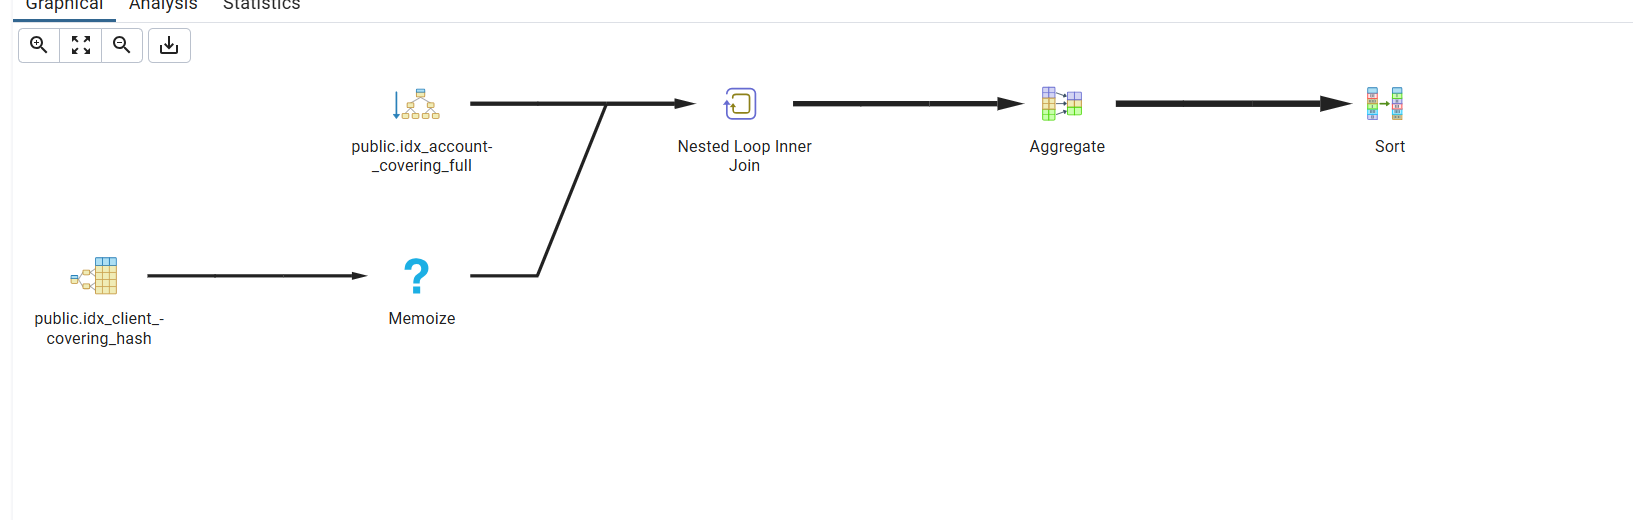
\includegraphics[width=1\textwidth]{Снимок экрана 2026-03-20 104940.png}
\end{figure}


\begin{figure}[H]
    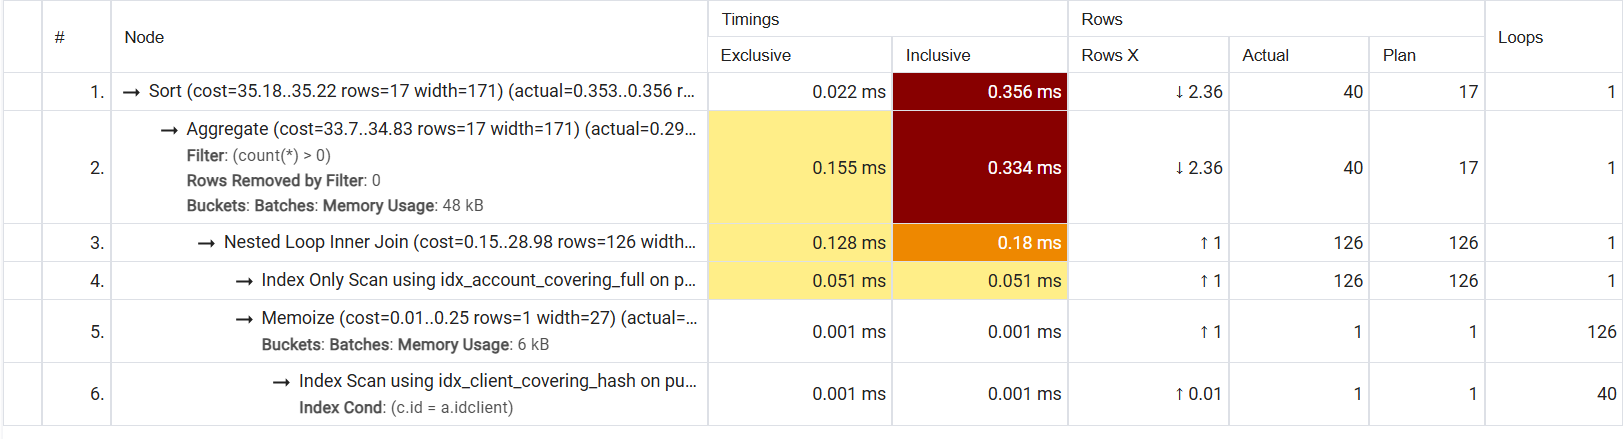
\includegraphics[width=1\textwidth]{Снимок экрана 2026-03-20 104909.png}
\end{figure}


    \subsection{Hash индекс с использованием выражений}


      \begin{verbatim}
  SELECT Name, LastName, PhoneNumber
FROM Client
WHERE Name IN ('Иван', 'Мария', 'Алексей', 'Елена');  
  \end{verbatim}

    \begin{figure}[H]
    
\includegraphics[width=1\textwidth]{Снимок экрана 2026-03-20 113120.png}
\end{figure}


\begin{figure}[H]
    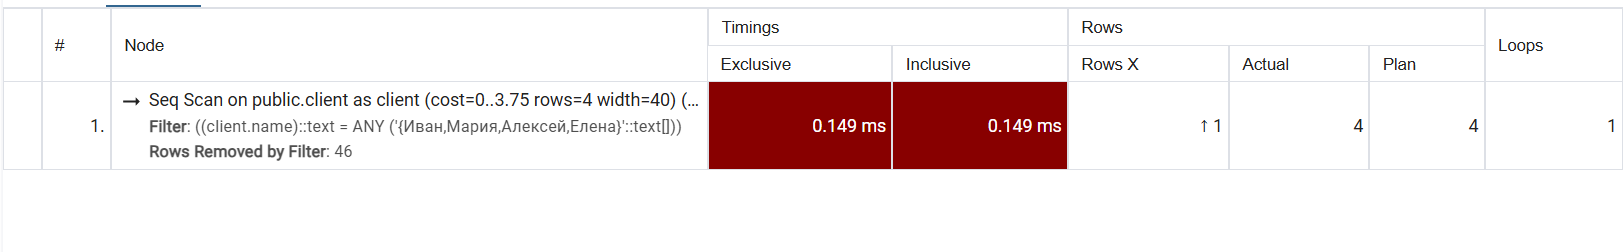
\includegraphics[width=1\textwidth]{Снимок экрана 2026-03-20 113045.png}
\end{figure}


  \begin{verbatim}
  CREATE INDEX idx_client_name_hash ON Client USING HASH(Name);  
  \end{verbatim}

  \begin{figure}[H]
    
\includegraphics[width=1\textwidth]{Снимок экрана 2026-03-20 103826.png}
\end{figure}


\begin{figure}[H]
    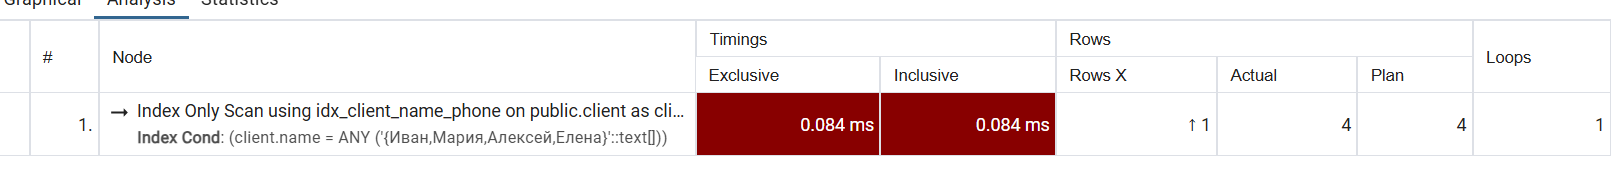
\includegraphics[width=1\textwidth]{Снимок экрана 2026-03-20 103742.png}
\end{figure}


    \subsection{Частичный Hash индекс}



  \begin{verbatim}
 SELECT Name, LastName, NumberPurchase,
    CASE 
        WHEN NumberPurchase BETWEEN 5 AND 15 THEN 'Постоянный клиент'    
        WHEN NumberPurchase BETWEEN 16 AND 25 THEN 'VIP-клиент'
        ELSE 'Супер-VIP'
    END AS ClientCategory
FROM Client
ORDER BY NumberPurchase DESC;   
  \end{verbatim}

    \begin{figure}[H]
    
\includegraphics[width=1\textwidth]{Снимок экрана 2026-03-20 121006.png}
\end{figure}


\begin{figure}[H]
    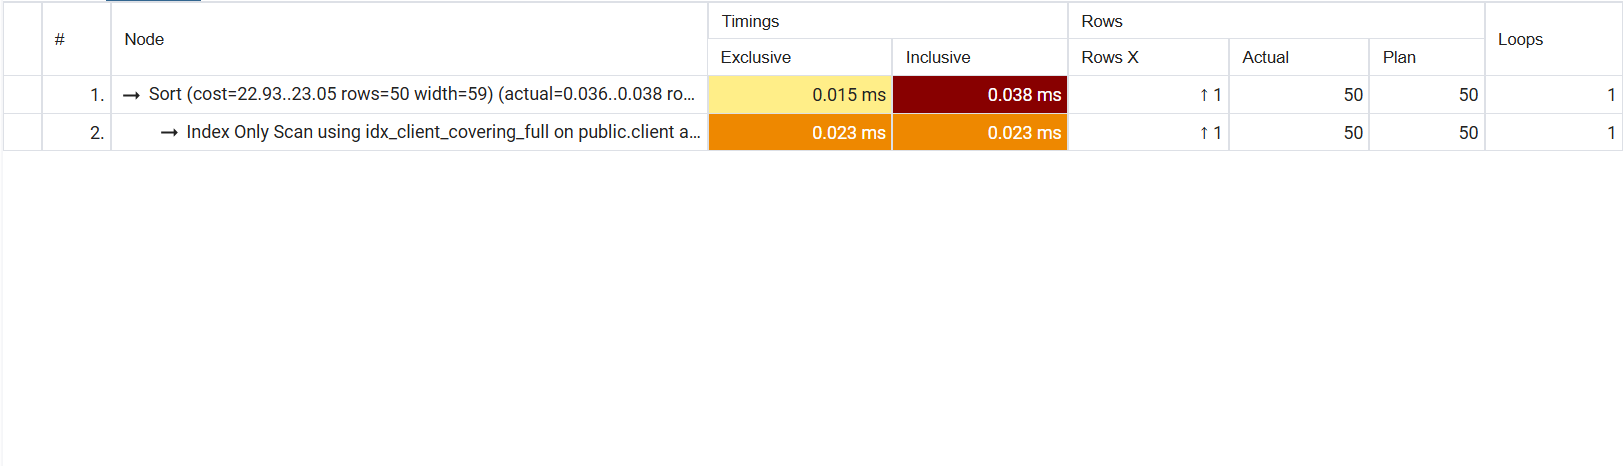
\includegraphics[width=1\textwidth]{Снимок экрана 2026-03-20 105721.png}
\end{figure}


  \begin{verbatim}
  CREATE INDEX idx_client_regular_name_hash ON Client USING HASH(Name) 
WHERE NumberPurchase BETWEEN 10 AND 20;  
  \end{verbatim}


  \begin{figure}[H]
    
\includegraphics[width=1\textwidth]{Снимок экрана 2026-03-20 105752.png}
\end{figure}


\begin{figure}[H]
    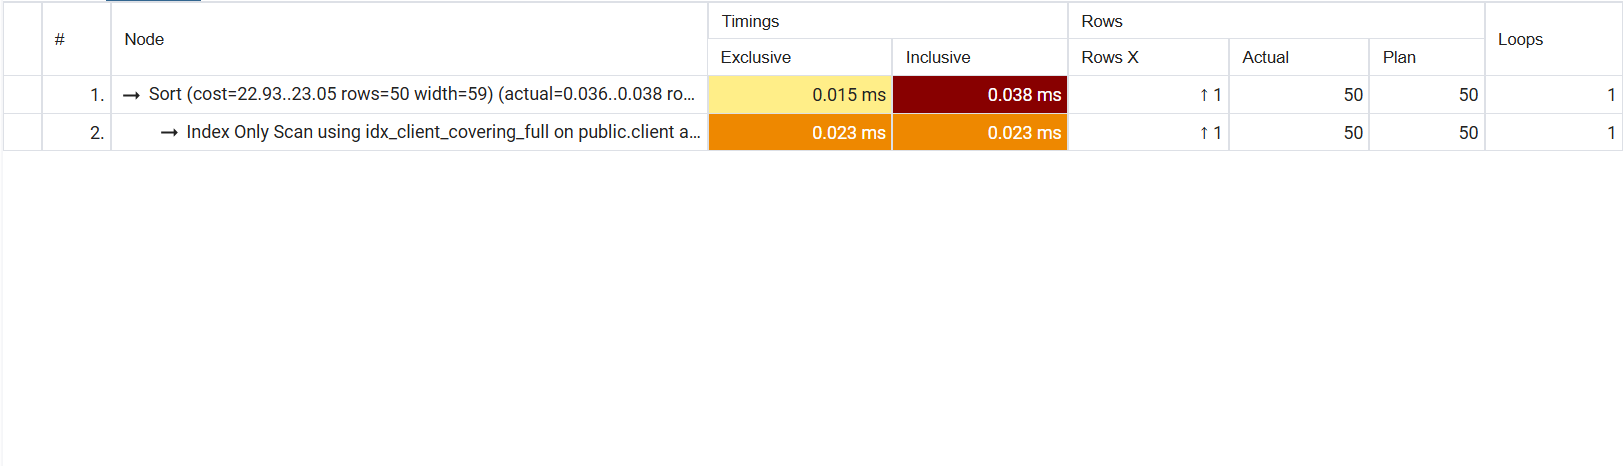
\includegraphics[width=1\textwidth]{Снимок экрана 2026-03-20 105721.png}
\end{figure}

   
    \appendix
     
\end{document}